\documentclass{article}

\usepackage{tikz}
\usetikzlibrary{decorations.pathreplacing}
\usetikzlibrary{fadings}

\begin{document}

\begin{figure}[h!]
	\centering
	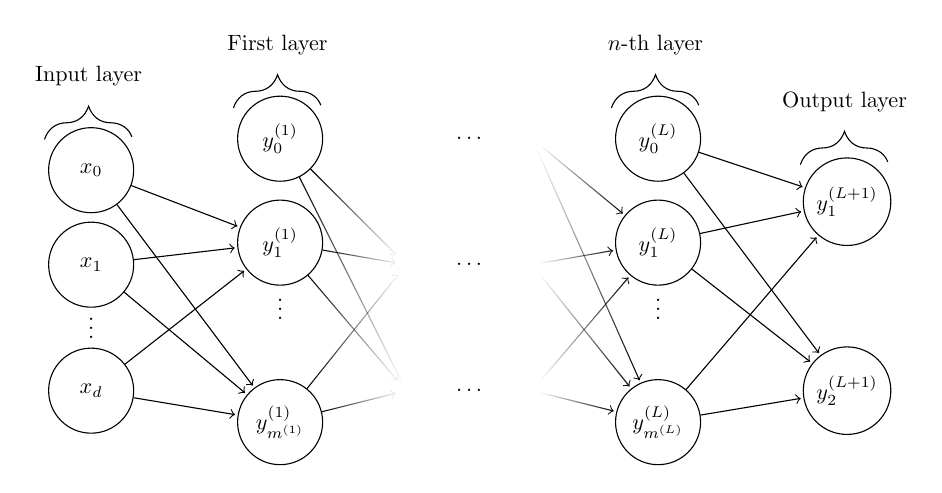
\begin{tikzpicture}[shorten >=1pt,scale=0.8, every node/.style={scale=0.8}]
	\tikzstyle{unit}=[draw,shape=circle,minimum size=1.35cm]
	\tikzstyle{hidden}=[draw,shape=circle,minimum size=1.35cm]
	
	\node[unit](x0) at (0,3.5){$x_0$};
	\node[unit](x1) at (0,2){$x_1$};
	\node at (0,1.1){\vdots};
	\node[unit](xd) at (0,0){$x_d$};
	
	\node[hidden](h10) at (3,4){$y_0^{(1)}$};
	\node[hidden](h11) at (3,2.35){$y_1^{(1)}$};
	\node at (3,1.4){\vdots};
	\node[hidden](h1m) at (3,-0.5){$y_{m^{(1)}}^{(1)}$};
	
	\node(h22) at (5,0){};
	\node(h21) at (5,2){};
	\node(h20) at (5,4){};
	
	\node(d3) at (6,0){$\ldots$};
	\node(d2) at (6,2){$\ldots$};
	\node(d1) at (6,4){$\ldots$};
	
	\node(hL12) at (7,0){};
	\node(hL11) at (7,2){};
	\node(hL10) at (7,4){};
	
	\node[hidden](hL0) at (9,4){$y_0^{(L)}$};
	\node[hidden](hL1) at (9,2.35){$y_1^{(L)}$};
	\node at (9,1.4){\vdots};
	\node[hidden](hLm) at (9,-0.5){$y_{m^{(L)}}^{(L)}$};
	
	\node[unit](y1) at (12,3){$y_1^{(L+1)}$};
	\node[unit](y2) at (12,0){$y_2^{(L+1)}$};
	
	\draw[->] (x0) -- (h11);
	\draw[->] (x0) -- (h1m);
	
	\draw[->] (x1) -- (h11);
	\draw[->] (x1) -- (h1m);
	
	\draw[->] (xd) -- (h11);
	\draw[->] (xd) -- (h1m);
	
	\draw[->] (hL0) -- (y1);
	\draw[->] (hL0) -- (y2);
	
	\draw[->] (hL1) -- (y1);
	\draw[->] (hL1) -- (y2);
	
	\draw[->] (hLm) -- (y1);
	\draw[->] (hLm) -- (y2);
	
	\draw[->,path fading=east] (h10) -- (h21);
	\draw[->,path fading=east] (h10) -- (h22);
	
	\draw[->,path fading=east] (h11) -- (h21);
	\draw[->,path fading=east] (h11) -- (h22);
	
	\draw[->,path fading=east] (h1m) -- (h21);
	\draw[->,path fading=east] (h1m) -- (h22);
	
	\draw[->,path fading=west] (hL10) -- (hL1);
	\draw[->,path fading=west] (hL11) -- (hL1);
	\draw[->,path fading=west] (hL12) -- (hL1);
	
	\draw[->,path fading=west] (hL10) -- (hLm);
	\draw[->,path fading=west] (hL11) -- (hLm);
	\draw[->,path fading=west] (hL12) -- (hLm);
	
	\draw [decorate,decoration={brace,amplitude=12pt},xshift=-4pt,yshift=-6pt] (-0.6,4.2) -- (0.8,4.2) node [black,midway,yshift=+1cm]{Input layer};
	\draw [decorate,decoration={brace,amplitude=12pt},xshift=-4pt,yshift=-6pt] (2.4,4.7) -- (3.8,4.7) node [black,midway,yshift=+1cm]{First layer};
	\draw [decorate,decoration={brace,amplitude=12pt},xshift=-4pt,yshift=-6pt] (8.4,4.7) -- (9.8,4.7) node [black,midway,yshift=+1cm]{$n$-th layer};
	\draw [decorate,decoration={brace,amplitude=12pt},xshift=-4pt,yshift=-6pt] (11.4,3.8) -- (12.8,3.8) node [black,midway,yshift=+1cm]{Output layer};
	\end{tikzpicture}
	\caption{Representation of a multilayer perceptron for binary classification of L+1 layers with an input vector of dimension $d$ and two output units where the hidden L-th layer contains m$^{(l)}$ neurons}
	\label{fig:multilayer-perceptron}
\end{figure}

\end{document}